%*******************************************************************************
%*********************************** First Chapter *****************************
%*******************************************************************************

\chapter{Introduction}  %Title of the First Chapter

Globally, there are approximately 80-100 tropical storms each year. The greatest frequency is observed in the Western North Pacific (WNP), with an average of 26 per year since 1981 \citep{zhan2012seasonal}. From 1977-2011, China had the highest rate of landfalls globally, averaging 6.4 per year \citep{HironoriFudeyasu:178}. Not only does the West Pacific experience the greatest number of tropical storms and landfalls per year, but also the most intense and largest. Tropical storms can occur throughout the year in the West Pacific, but the most active season is June-November.

%********************************** %First Section  **************************************

\section{Characteristics of tropical storms}

A tropical storm is a low pressure system that forms over tropical or sub-tropical waters (i.e. 23.4$^{\circ}$N to  23.4$^{\circ}$S), with organised convection and winds at low levels circulating anti-clockwise in the northern hemisphere or clockwise in the southern hemisphere. 

\begin{figure}[h]
	\centering
	\noindent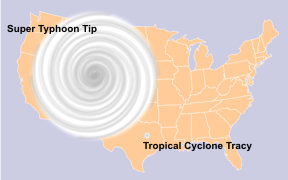
\includegraphics[width=15pc,angle=0]{H:/Documents/Admin/ESA/Figures/typhoonsizes.jpg}
	\caption{Comparison of tropical cyclone sizes: Super Typhoon Tip and Tropical Cyclone Tracy. Source: \cite{noaa_structure}}\label{fig:cyclone_size}
\end{figure}

They are hugely variable in terms of size, illustrated in figure \ref{fig:cyclone_size}, where Tropical Cyclone Tracy (1974) covers just 0.03\% the area of Super Typhoon Tip (1979). Tropical cyclones tend to extend throughout the depth of the troposphere, approximately 16 km. The Saffir-Simpson Hurricane Scale \citep{simpson1974hurricane} is often used to categorise tropical storms by intensity based on maximum winds. Storms with winds of 38 mph (61 km/h, 33 knots) or less are called 'tropical depressions' and above this they are called 'tropical storms'. With increasing intensity there are categories 1 to 5 'hurricanes', with categories 3,4,5 referred to as 'major hurricanes'. In the West Pacific basin, if maximum sustained winds reach 64 knots (33 m/s, 74 mph) the term 'typhoon' is used, and a 'Super Typhoon' is if the maximum sustained winds are at least 130 knots (67 m/s, 150 mph).
The speed they move along the underlying surface, or 'translation speed' is around 10-15mph (10 knots), but can slower or as fast as 40 mph \citep{mo_tc}.  
%Size is not necessarily an indication of hurricane intensity. 


\subsection{Formation of tropical storms}

There are a number of environmental factors that need to be satisfied in order for a tropical storm to generate at a location. These are:
\begin{itemize}
	\item Presence of a convective system
	\item Non-negligible Coriolis force (at least 500 km, 300 miles) from the equator) \citep{noaaA15}
	\item Low wind shear (less than about 20 knots (10 m/s, 23 mph) \citep{noaaA15} 
	%	\item Enhanced vorticity
	\item Sufficient humidity in the mid-troposphere
	\item Warm ocean water of at least 26.5$^{\circ}$C throughout a sufficient depth (50m) (section 1.3.1)
	
\end{itemize}

Tropical cyclones cannot be generated spontaneously. To develop, they require a weakly organized system with sizeable spin and low level inflow. For tropical cyclogenesis to occur, there is a requirement for the Coriolis force to provide for near gradient wind balance to occur. Without the Coriolis force, the low pressure of the disturbance cannot be maintained. Large values of vertical wind shear disrupt the incipient tropical cyclone and can prevent genesis, therefore little wind shear is important. Relatively moist layers near the mid-troposphere (5 km, 3 miles). Dry mid levels are not conducive for allowing the continuing development of widespread thunderstorm activity. The development and maintenance of tropical cyclones require a warm ocean surface to act as a source of energy.

%Tory = enhanced cyclonic low-level vorticity .A pre-existing near-surface disturbance with sufficient vorticity and convergence. 
%Tropical waves spawn tcs... AEW, MT
%An atmosphere which cools fast enough with height such that it is potentially unstable to moist convection. 
%Tory - Tory - deep convection


\subsection{Tropical storm structure}

The main parts of a tropical cyclone are the dense cirrus overcast, rainbands, the eye, and the eyewall (figure \ref{fig:cyclone_structure}). There is boundary layer inflow in a cyclonic direction (anti-clockwise in the northern hemisphere) and anti-cyclonic (clockwise) upper tropospheric outflow.


\begin{figure}[h]
	\centering
	\noindent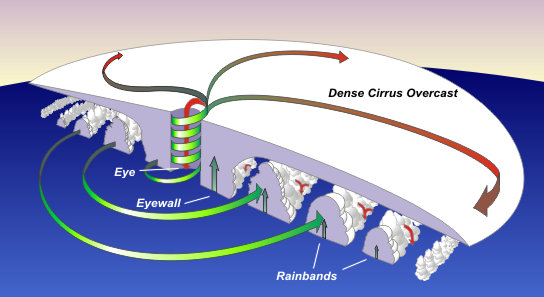
\includegraphics[width=20pc,angle=0]{H:/Documents/Admin/ESA/Figures/hurr_cross.jpg}
	\caption{Tropical cyclone structure. Source: \cite{noaa_structure}}\label{fig:cyclone_structure}
\end{figure}

\subsubsection{Eye and eye wall}
The circular 'eye' or centre of a tropical cyclone is an area of slowly sinking air, characterised by light winds (usually do not exceed 15 mph (24 km/h)) \citep{noaa_structure} and little or no precipitation (figure \ref{fig:cyclone_structure}). Eye diameters are typically 40 km but can range from under 10 km to over 100 km \citep{bom_tc}. Although the winds are calm at the axis of rotation, strong winds may extend well into the eye. The eye is the region of lowest surface pressure and warmest temperatures aloft.

\begin{figure}[h]
	\centering
	\noindent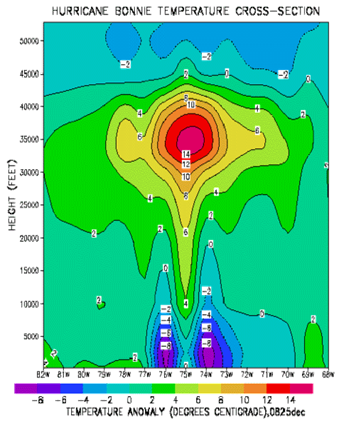
\includegraphics[width=14pc,angle=0]{H:/Documents/Admin/ESA/Figures/warm_core2.png}
	\caption{Hurricane Bonnie temperature cross-section: the warm core. Source: \cite{eastin}}\label{fig:warm_core}
\end{figure}

Figure \ref{fig:warm_core} shows the maximum temperature anomalies present in the upper levels of the eye of Hurricane Bonnie. This is a result of subsidence and adiabatic heating in the eye, and eyewall latent heat release. The warm core is responsible for the extremely low surface pressures in the eye and large pressure gradients across the eyewall. The eye temperature may be 10$^{\circ}$C warmer or more at an altitude of 12 km (8 miles) than the surrounding environment, but only 0-2$^{\circ}$C warmer at the surface (Hawkins and Rubsam 1968) in the tropical cyclone (figure \ref{fig:warm_core}).

The eye is surrounded by a dense ring of cloud deep convection about 16 km high known as the eye wall which marks the belt of strongest winds and heaviest rainfall (\citep{bom_tc}). Changes in the structure of the eye and eyewall can cause affect the wind speed within the storm. The eye can grow or shrink in size, and double (concentric) eyewalls can form. In intense tropical cyclones, some of the outer rainbands may organize into an outer ring of thunderstorms that slowly moves inward. The inner eye wall (and storm intensity) weakens as it feels the effects of the subsidence resulting from this outer eyewall, inhibiting the inner eyewall of its needed moisture and momentum. Eventually the outer eyewall replaces the inner one completely and the storm can be the same intensity as it was previously or, in some cases, even stronger.% REF this section about weakening and intensifying. The pressure rises due to the destruction of the inner eyewall are usually more rapid than the pressure falls due to the intensification of the outer eyewall, and the cyclone itself weakens for a short period of time. 
%Some of the most intense tropical cyclones exhibit concentric eyewalls, two or more eyewall structures centered at the circulation center of the storm ( Willoughby et al. 1982,Willoughby 1990a ). Just as the inner eyewall forms, convection surrounding the eyewall can become organized into distinct rings. 

There remains some debate about the mechanism by which the eye forms \citep{noaa_a11}. It may be due to the downward directed pressure gradient associated with the weakening and radial spreading of the tangential wind field with height (Smith, 1980), or subsidence forced by latent heat release in the eye wall (Shapiro and Willoughby, 1982), or a combination of mechanisms.

%The exact mechanism by which the eye forms remains somewhat controversial. One idea suggests that the eye forms as a result of the . Another hypothesis suggests that the eye is formed when latent heat release in the eyewall occurs, forcing subsidence in the storm's center . It is possible that these hypotheses are not inconsistent with one another. In either case, as the air subsides, it is compressed and warms relative to air at the same level outside the eye and thereby becomes locally buoyant. This upward buoyancy approximately balances the downward directed pressure gradient so that the actual subsidence is produced by a small residual force.  \citep{noaa_a11}

%At around 74 mph (119 km/h) the strong rotation of air around the cyclone balances inflow to the center, causing air to ascend about 10-20 miles (16-32 km) from the center forming the eyewall. This strong rotation also creates a vacuum of air at the center, causing some of the air flowing out the top of the eyewall to turn inward and sink to replace the loss of air mass near the center.

\subsubsection{Rain bands}
Convection in tropical cyclones is organized into long, narrow rainbands which are oriented in the same direction as the horizontal wind (figure \ref{fig:cyclone_structure}). Along these bands, low-level convergence and upper-level divergence are at a maximum. Warm, moist air converges at the surface, ascends through these bands, diverges aloft, and descends on both sides of the bands. Subsidence is distributed over a wide area on the outside of the rainband but is concentrated in the small inside area \citep{noaa_a11}. As the air subsides, adiabatic warming takes place, and the air dries. Because subsidence is concentrated on the inside of the band, the adiabatic warming is stronger inward from the band causing a sharp contrast in pressure falls across the band since warm air is lighter than cold air. Because of the pressure falls on the inside, the tangential winds around the tropical cyclone increase due to increased pressure gradient and eventually the band moves towards the centre (Willoughby 1979, 1990a, 1995). 

% Eventually, the band moves toward the center and encircles it and the eye and eyewall form 

%What is the intensity of rain in a TC?


\subsection{Tropical cyclone energy and lifecycle}

Within a tropical cyclone, there are two distinct circulations referred to as 'primary' and 'secondary' (figure \ref{fig:cyclone_circ}). The primary circulation is what visibly characterises the phenomenon, with winds swirling cyclonically around the cyclone eye. The secondary circulation is the flow of air into the centre, ascending in the eye and then divergence at upper levels.

%\begin{figure}[h]
%	\centering
%	\noindent\includegraphics[width=20pc,angle=0]{H:/Documents/Admin/ESA/gradient_wind_balance.png}
%	\caption{Gradient wind balance in primary circulation of a tropical cyclone. Source: \cite{circ_pic}}\label{fig:cyclone_circ}
%\end{figure}
%% Do not cite circ_pic as this reference url has '%', which means all following references are missed

\subsubsection{Gradient wind balance}% and thermal wind balance}

The basic horizontal balance in a tropical cyclone above the boundary layer is between the sum of the Coriolis and centripetal forces, balanced by the horizontal pressure gradient force. This balance is referred to as gradient balance (figure \ref{fig:cyclone_circ}). %The centripetal force alters the original two-force geostrophic balance and creates a non-geostrophic gradient wind.
The classic theory for hurricane intensification relies on the inflow induced by the deep convection. However, as the vortex strengthens, the boundary layer becomes increasingly important \citep{under_hurr}.

%A symmetric tropical cyclone is in approximate thermal wind balance \citep{comet_tm}. The thermal wind is the difference between the geostrophic wind at two vertical levels and therefore represents the vertical wind shear of the geostrophic wind.

%what goes on in the boundary layer?
%http://www.goes-r.gov/users/comet/tropical/textbook_2nd_edition/navmenu.php_tab_9_page_2.4.1.htm

%The reason that different peak winds can result in different central pressures is caused by the fact that the radius, r, of the peak wind varies. A storm with 40 m/s peak winds with a 100 km RMW will have a much lower pressure drop than one with a 25 km RMW.

\begin{figure}[h]
	\centering
	\subfloat[1a]{\includegraphics[width=2.4in]{H:/Documents/Admin/ESA/Figures/gradient_wind2006.png}}
	\subfloat[2a]{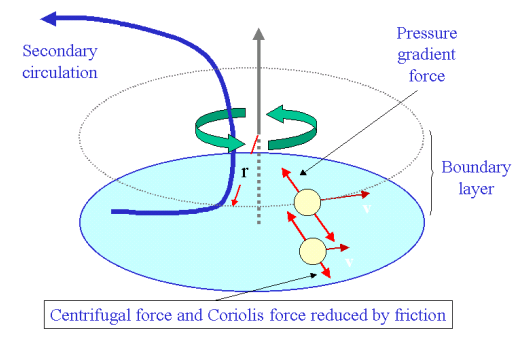
\includegraphics[width=2.4in]{H:/Documents/Admin/ESA/Figures/gradient_wind2006B.png}}
	
	%	\noindent\includegraphics[width=20pc,angle=0]{H:/Documents/Admin/ESA/gradient_wind2006.png}
	\caption{a) gradient wind force balance in the primary circulation of a tropical cyclone b) disruption of gradient wind balance by friction in the boundary layer leaving a net inward pressure gradient that drives the secondary circulation with inflow in the boundary layer and outflow above it. Source: Smith, 2006}\label{fig:cyclone_circ}
\end{figure}

Surface friction in the boundary layer reduces the wind speed near the surface and therefore the centrifugal and Coriolis forces, but has little effect on the pressure field. There is therefore a new inward force in the boundary layer, driving inflow and the secondary circulation. The conservation of angular momentum means is objects will spin faster as they move toward the centre of circulation, so air increases its speed as it heads toward the centre of the tropical cyclone.


\subsubsection{Potential intensity}

To a good approximation, the secondary circulation in a tropical cyclone is a natural realisation of a Carnot heat engine, except that the engine does no work on its environment, the available work is locally dissipated and a fraction of the dissipated energy is recycled into the engine. A Carnot heat engine is the most efficient heat engine cycle allowed by physical laws. The Carnot perspective provides an upper bound on the maximum wind speed that a storm can attain.

\begin{figure}[h]
	\centering
	\noindent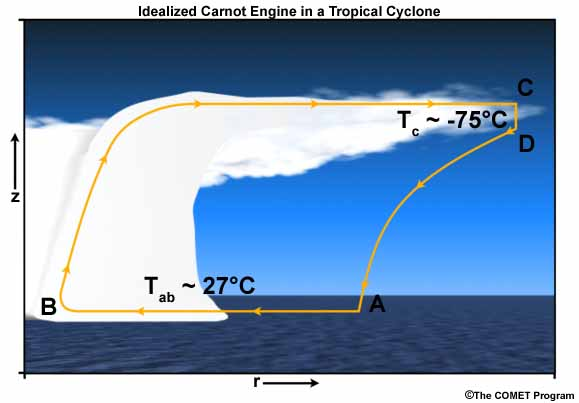
\includegraphics[width=20pc,angle=0]{H:/Documents/Admin/ESA/Figures/carnot1.jpg}
	\caption{The Carnot cycle in a tropical cyclone. A-B: isothermal inflow of near-surface air; B-C: moist adiabatic ascent in the eye wall and outflow just below the tropopause; C-D: sinking of cooled air in the environment far from the tropical cyclone center. To close the system, D-A: the cooled air is assumed to return to the tropical cyclone environment adiabatically. Source:\cite{goescarnot}}\label{fig:cyclone_carnot}
\end{figure}

%CISK / WISHE
%\cite{emanuel1991theory} ref for carnot cycle
%vortical hot tower

%As this air ascends, 90\% of the stored energy is released by condensation, giving rise to the towering cumulus clouds and rain. The release of heat energy warms the air locally, causing a further decrease in pressure aloft. Consequently, air rises faster to fill this area of low pressure, and more warm, moist air is drawn off the sea, feeding further energy to the system. Thus, a self-sustaining heat engine is created.
%As little as 3\% of the heat energy may be converted into mechanical energy of the circulating winds. This relatively small amount of mechanical energy equates to a power supply of 1.5x1012 Watts - equivalent to about half the world-wide electrical generating capacity!
%http://www.metoffice.gov.uk/weather/tropicalcyclone/facts
%Emanuel theory 
%static vs dynamic theory

%In the northern hemisphere, positive vorticity at low levels and negative at upper levels. Vorticity decays with height. 

%It is the thunderstorm activity which allows the heat stored in the ocean waters to be liberated for the tropical cyclone development. (deep surface layer of conditional instability) - see Tory

%Intensification and decay
%Large vertical shear can weaken or destroy the tropical cyclone by interfering with the organization of deep convection around the cyclone center.
%(noaa website)
%maturity

%gray, frank montgomery, smith, tory book chapter- number of environmental conditions require to be satisfied for tc genesis.
%Emanuel
%ventilation
%Warm core is in thermal wind balance with the primary circulation.


\subsection{Steering of tropical storms} \label{steer}



%rotating winds of a tropical cyclone, combined with the north–south variation in the Coriolis parameter, induce relative vorticity asymmetries in the tropical cyclone (Fig. 8.60). These asymmetries are called the β–gyres.
%Tropical cyclones move in relation to the integrated, deep-layer (to \textasciitilde 17 km) environment flow in which they are embedded \citep{neumann1985role}.
% annulus degrees = see Carr 
%The motion of a tropical cyclone is highly correlated with latitude \citep{neumann1985role}. 
%5Chan 1985. (ref atm and ocean control sections). Low latitude easterlies and high lat westerlies, subtropical high.

A tropical cyclone is approximately 500-1000 km wide and 10-16 km high, set in much larger scale flow, so it can be treated as a solid object floating in the atmosphere \citep{chan2005physics}. Environmental steering is typically defined as the wind within an annulus centred on the tropical cyclone. e.g. 5-7 degrees (\citep{chan1982tropical}, \citep{chan1985identification} or 3 degrees (Franklin 1996). To define the steering flow, tropospheric layer means are better than single-level analyses \citep{velden1991basic}, with the deep layer mean (DLM)(1000-100 hPa) or mid-tropospheric level (500-700 hPa) often used. The vector quantity for the difference between the environmental steering and tropical cyclone motion is termed 'propagation' \citep{carr1990observational}. This difference arises from variations in the Coriolis parameter and environmental vorticity across the tropical cyclone. 

Depending on direction of movement of the storm, there is a different relationship with the surrounding flow \citep{chan1985identification}. Westward moving TCs move faster and to the left of the steering in the Northern Hemisphere, and eastward moving TCs move slower and to the right \citep{carr1990observational}.
%Importance of zonal direction of cyclone translation in determining the relationship between the environmental flow and cyclone movement. 

%Steered by surrounding flow and modified by Coriolis force (beta effect) and the horizontal vorticity gradient of the surrounding flow (chan physics review).
%NH Tcs move 10-20 degrees to the left and faster by 1ms than mid-tropospheric (700, 600, 500) at 6 degrees. 
%The beta effect - the cyclone and environment interact to modify the basic flow, and the vortex is then steered by this modified flow.

Studies have shown that depth of the steering layer is related to the strength of the cyclone \citep{velden1991basic}. For a more intense storm, there is greater vertical development of the cyclonic vortex, which is then advected by an environmental flow of greater depth. 

Tropical cyclone translation after landfall is affected by terrain, circulation environment, steering flow, TC intensity and structure among others \citep{xiao2013analysis}.
% effects of land, e.g. Philippines, Taiwan. track variation - interaction with topography (Wu and Kuo 1999), Taiwan


%Previous investigation into the sudden change in tropical cyclone track in four storms in the WNP suggested that such changes occurred near the centre of the MJO-scale cyclonic circulation or at the birfurcation of steering flows at 700 hPa \citep{wu2011observational}.

%Tropical cyclones forming between 5 and 30 degrees North latitude typically move toward the west. Sometimes the winds in the middle and upper levels of the atmosphere change and steer the cyclone toward the north and northwest. When tropical cyclones reach latitudes near 30 degrees North, they often move northeast

%Kim et al MJO effect
%Monsoon trough effect


\section{Impact of tropical storms}

Tropical cyclones are the most devastating natural hazards, affecting large populations in both the developed and developing world. Most of the damage occurs when tropical cyclones make landfall, and it is not only the destructive force of the strong winds, but also heavy precipitation and storm surge that cause widespread damage to communities.

Storm surges are responsible for much of the damage associated with landfalling tropical cyclones \citep{lin2012physically}. Storm surge is complicated, determined by the characteristics of the storms as well as shape and bathymetry of the coast, and the importance of the storm characteristics whilst over the open ocean and before landfall are also important. Rainfall distribution and intensity is complicated and depends on interactions on a variety of scales, with track, intensity, topography and environmental vertical shear all having an impact. Tropical storm wind fields change drastically when they make landfall, involving a complex interaction with the system and the underlying surface. The maximum damage of a tropical cyclone is not always at the point of landfall, but can be when it is further inland, for example when heavy rainstorms caused by interaction with mid-and lower-latitude systems once the storm is overland occur \citep{xiao2013analysis}. Although most damage occurs when tropical storms make landfall, they can also cause significant damage whilst at sea, mainly to the offshore industry. Loading on offshore structures is a complex function of not only characteristics of the wind field but also ocean characteristics including currents and waves \citep{done2014future}. Tropical-cyclone-wind resistant turbines have been deployed off the coast of China \citep{clark2014global}, to increase resilience to any future storms.

A recent notable tropical storm in the Western North Pacific is Super Typhoon Haiyan (2013). This is one of the most powerful typhoons ever to make landfall, with maximum sustained winds of 170 knots (88 m/s, 195 mph). Haiyan tracked over the Philippines archipelago, with storm surge primarily responsible for 6,300 dead, 1061 missing and almost 30,000 injured \citep{lagmay2015devastating}. %Average 472 fatalities a year (1983-2006) \citep{zhang2009tropical} 

Such landfalling typhoons also have a significant economic impact, for example Super Typhoon Herb (1996) caused 73.26 billion yuans  (£8.31 billion) in direct economic losses and became the costliest landfalling tropical cyclone in China at the time \citep{zhang2009tropical}. In China, there is an upward trend in the economic cost of landfalling tropical cyclones, and this is principally caused by economic development \citep{zhang2009tropical}.

%http://www.air-worldwide.com/Press-Releases/AIR-Estimates-Insured-Losses-from-Super-Typhoon-Haiyan-at-Between--USD-300-Million-and-USD-700-Million/

% From zhang2009tropical: In an average year, landfalling tropical cyclones cause 472 deaths and 28.7 billion yuans (2006 RMB) in direct economic losses, accounting for 0.38% of the annual total gross domestic product (GDP) of China. As the deadliest landfalling tropical cyclone, Super Typhoon Fred killed 1,126 people in 1994, making it the deadliest year (1,815 deaths). The costliest landfalling tropical cyclone was Super Typhoon Herb, which caused 73.3 billion yuans (2006 RMB) in direct economic losses in 1996, making it the costliest year (107.9 billion yuans). The direct economic losses and casualties of a landfalling tropical cyclone tend to increase with the northward shift in landfall track.



%%%%%%%%%%%%%%%%%%%%%%%%%%%%%%%%%%%%%%%%%%%%%%%%%%%%%%%%%%%%%%%%%%%%%%%%%%%%%%%%%%%%%%%%%%%%%%%%%%%%%%%%
\section{Tropical storm activity}

The Saffir-Simpson Hurricane Scale \citep{simpson1974hurricane} is often used to categorise tropical storms by intensity. Storms with maximum sustained winds of 38 mph (61 km/h, 33 knots) or less are called 'tropical depressions' and once over this threshold, are called 'tropical storms'. In the West Pacific basin, if maximum sustained winds reach 64 knots (33 m/s, 74 mph) the term 'typhoon' is used, and a 'Super Typhoon' is if the maximum sustained winds are at least 130 knots (67 m/s, 150 mph). %(http://www.srh.noaa.gov/jetstream/tropics/tc\_classification.html)
%(I need to remember if 1-min or 10-min. Which is US? Which is WMO?)

\subsection{Influence of the ocean} \label{ocean}

The ocean provides a source of energy to the tropical cyclone system by air-sea sensible and latent heat fluxes, determined by the sea surface temperature (SST). Many studies have shown that the SST must exceed 26$^{\circ}$C for tropical cyclones to form \citep[e.g.][]{palmen1948formation}. However, there is much research into this threshold \citep[e.g.][]{dare2011threshold, mctaggart2015revisiting}, highlighting basin-dependence and the importance of ocean temperature below the sea surface. The WNP has high SST throughout the year (\textgreater 28.5$^{\circ}$C) \citep{chan2007interannual}, relative to the suggested 26.5$^{\circ}$C threshold for genesis (section 1.2.1). Variability in activity is related to the SST pattern, with warm anomalies favouring intensification. The West Pacific is warm, past threshold limit, threshold more suitable for the North Atlantic, where more marginal.

The potential intensity of a tropical cyclone is directly related to the SST below the cyclone, all else being equal \citep{emanuel1991theory, holland1997maximum}, with higher SST promoting increased intensity. At high wind speeds, the surface wind stress generates strong turbulent mixing within the ocean. This causes entrainment of cooler water towards the surface from the thermocline and deepens the mixed layer.  The cooling of the SST is determined by the initial state of ocean, storm intensity, translation speed and storm size, and limits storm intensification, especially for slow moving storms, where SST cools more \citep{bender1993numerical, bender2000real}. During the lifetime of a storm, the wake produced can change considerably, for example Megi (2010) created a wake of 1.6$^{\circ}$C whilst in the Philippine Sea, but once in the South China Sea, cooling increased greatly to 7$^{\circ}$C \citep{d2014impact}. Due to this turbulent entrainment of cold water into the oceanic mixed layer induced by the TC, the state of ocean below the surface is also important to the cyclone system \citep{bender2000real, shay2000effects}.
%(see if any emanuel refs here - environmental control on...)
%Price 1981 - cooling 1 to 6C. \citep{price1981upper}
%Using satellites, observations of this cooling has been possible, 
%Cold wake of ~6C \citep{prasad2007upper}. 
%check Bender2000real.
%SST decrease induced by passage of a TC is approximately 1-6$^{\circ}$C  \citep{price1981upper}. 

The ocean heat content (OHC) in Joules (J) is a measure of the heat content within the ocean between two reference levels. 

\begin{equation}
OHC = c_{p} \int_{z1}^{z0} (T-T_{ref}) \rho dz
\end{equation} 	
%https://www.sharelatex.com/learn/Mathematical_expressions

%\begin{equation}
%$\displaystyle OHC = c_{p} \int_{z1}^{z0} (T-T_{ref}) \rho dz$
%\end{equation} 	

Tropical cyclone heat potential (TCHP) is vertically integrated heat content from the sea surface down to the 26$^0$C isotherm, which as at depth 'D26'.
% cannot find ref: as Gray (1968, 1978) suggested that depth of 60m is necessary for intensification.
%When this heat content is from the surface down to the 26$^0$C isotherm, it is termed tropical cyclone heat potential %(TCHP).
%Increased availability of sub-surface ocean observations, e.g. ARGO floats, since ...
%The ocean is the source of energy for a TC's intensification, typically down to 100-200m is important (Emanuel 1999) \citep{bender2000real}, \citep{shay2000effects}.
%Although WPAC SST is warm (generally above xyz), anomalously warm water can favour intensification. 

If the ocean warm layer (D26) is relatively shallow, (e.g. 60m) a positive SST anomaly is critical to intensification because the features can effectively deepen the warm layer and restrict the TC-induced cooling. If this layer is deep, e.g.\textgreater 105m, a warm feature is not required as the background is already sufficient to overcome the negative cooling feedback \citep{lin2008upper}.
%But isnt the warm SST anomaly needed in the first place?

In the WNP, intensification to category 5 needs SST around 29$^0$C and subsurface heat content required depends on the storm translation speed \citep{lin2009upper}. A shallow warm subsurface (D26 \textasciitilde 60m) is sufficient to intensify to a category 5 in a fast moving storm, but for slow moving storms, a much deeper warm layer is required \citep{lin2009upper}.

%Rapidly moving storms with deep oceanic mixed layer, SST feedback is of minor importance \citep{schade1999ocean}. All hurricanes attain their maximum intensity over warm ocean waters (does this mean the warmest or just above a threshold??) - from Prasad, referencing Goni and Trinanes, 2003

Typhoon Imbudo (2003) intensified from 56 knots (29 m/s, 65 mph) to 113 knots (58 m/s, 130 mph) in 12 hours when it passed over a region that increased TCHP by 100 kJ/cm$^2$. As the typhoon passed over these waters, the SST decreased by 3-4$^0$C alongside TCHP, but there was sufficient energy to negate the negative feedback of upwelling of cooler waters \citep{goni2003ocean}.
%But still there was cooling?


%On a much smaller scale, breaking waves and sea spray produced by TCs may change the wind stress \citep{moon2004effect}. Surface waves are a source of surface friction, moisture flux and ocean mixing and are a non-linear function of fetch and wind speed.

%Breivik et al. (2015) recently have demonstrated substantial improvement in climatological ocean biases with explicit treatment of surface waves. Waves generated by tropical cyclones are an important cause of infrastructure damage so an explicit and coupled treatment is desirable.

%%%%%%%%%%%%%%%%%%%%%%%%%%%%%%%%%%%%%%%%%%%%%%%%%%%%%%%%%%%%%%%%%%%%%%%


\subsection{Influence of the atmosphere}
%The atmosphere can maintain the TC or destroy it, principally through vertical wind shear.
A cyclone exists throughout the depth of the troposphere and so the atmospheric conditions have a large effect on the phenomenon. It has been established that vertical wind shear is detrimental to tropical cyclone genesis and intensification \citep[e.g.][]{chan1982tropical, McBride1995}, although mature, large tropical storms may resist relatively large wind shear \citep{zeng2007environmental}.

%One hypothesized pathway by which vertical shear affects tropical cyclones is mid-level ventilation, or the flux of low-entropy air into the centre of the tropical cyclone \citep{McBride1995}. Tropical upper tropospheric trough (TUTT) cells from the mid-latitudes can weaken tropical cyclones by introduction of vertical wind shear, but also bring a cyclonic PV anomaly, which may contribute to intensification \citep{zeng2007environmental}.
%EXPLAIN
%Strong vertical wind shear prohibits rapid intensification and most likely results in the weakening of TCs \citep{zeng2007environmental}.
%and a threshold of 12.5 ms$^-1$ above which TCs cannot form in the WPAC has been suggested \citep{zehr1992tropical}-seems to be a thesis - check this ref
%e and Zehr 1991, Zehr 1992 - thesis?)
%check zeng paper
% McBride and Tang for ventilation

The translation of TCs is largely determined by the large-scale atmospheric pattern, with mid-tropospheric levels (500 and 700 hPa) found to have the best correlation with TC direction and speed \citep{chan1982tropical} (\ref{steer}). If the passage of the storm is too slow, the cooling induced by the storm will inhibit intensification, and if it is moving too fast, the resulting asymmetric structure will also inhibit intensification \citep{zeng2007environmental}. Rapid intensification (RI) is An increase in the maximum sustained winds of a tropical cyclone of at least 30 kt in a 24-h period (\citep{nhc_gloss}). and for this to occur, a translation speed between 3-8 m/s is required. % (REF). % ref missing here

Although wind is the primary atmospheric control on TC activity, relative humidity and vorticity are also important.

% Fast translation speed and strong vertical shear and detrimental to TC intensification \citep{zeng2007environmental} and

%%%%%%%%%%%%%%%%%%%%%%%%%%%%%%%%%%%%%%%%%%%%%%%%%%%%%%%%%%%%%%%%%%%%%%%
\subsection{Tropical storm variability in the West Pacific}

Changes in atmospheric and oceanic conditions drive tropical cyclone variability. Tropical cyclone activity in most ocean basins including the WNP has a strong interannual signal \citep{landsea2000climate}, with variability observed in genesis location, track, intensity, landfall and lifetime.% (could use zhan2011contributions).

%Regions preferable for genesis. Or something like, genesis location is important and atmospheric conditions to maintain or dissipate storms are important. Distribution of SST important, also ocean at depth is important.

%(At the end mention interdecadal seasonal variability)

\subsubsection{El Ni\~{n}o}

It has been long established that the El Ni\~{n}o-Southern Oscillation (ENSO) (figure \ref{fig:nino}) is the principal driver of interannual variability in the Tropics. This phenomenon also has a marked effect on tropical storm activity in all basins. In a warm El Ni\~{n}o year, when the SST in the central and eastern equatorial Pacific is anomalously warm, there is a zonal displacement of annual mean tropical storm genesis location eastward \citep{lander1994exploratory, zhan2011contributions}. These storms tend to have a longer lifetime and can reach higher intensities before they recurve or meet land \citep{camargo2007cluster, chan1998seasonal}. In contrast, during La Ni\~{n}a years, the main region of genesis shifts westwards, with fewer intense storms.
%El Nino -weakening of Walker circulation. La Nina - strengthening.
%, Chan 2000, Wang and Chan 2002, for zonal displacement ENSO.


\begin{figure}[h]
	\centering
	\noindent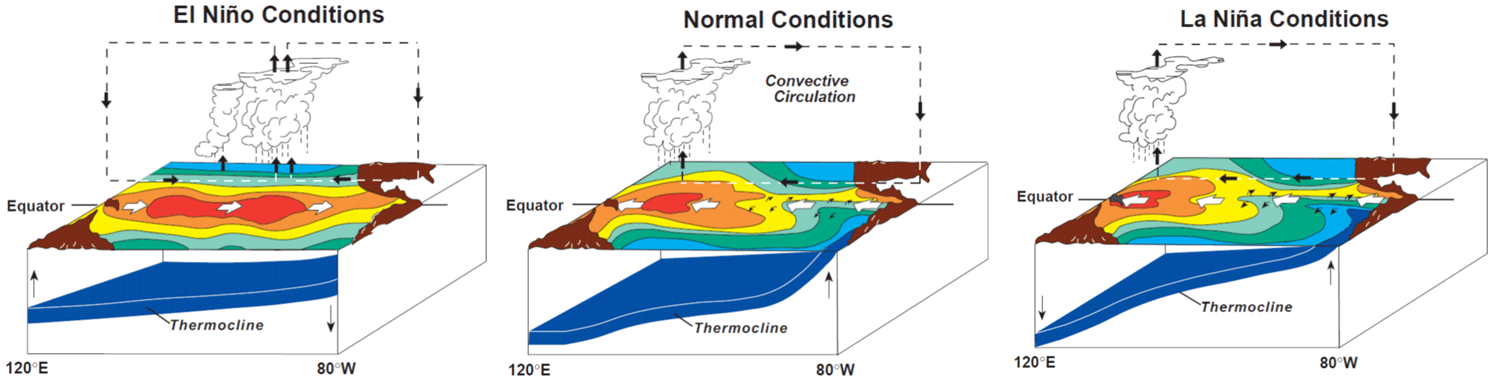
\includegraphics[width=40pc,angle=0]{H:/Documents/Admin/ESA/Figures/Stressors_ENSO3.png}
	\caption{El Ni\~{n}o, normal and La Ni\~{n}a conditions in the atmosphere and ocean in the tropical Pacific. Source: \cite{noaa_enso}}\label{fig:nino}
\end{figure}


There is a significant difference in landfall location between El Ni\~{n}o and La Ni\~{n}a years. During El Ni\~{n}o, with more storms generated in the southeast quadrant of the WNP, they tend to recurve before landfall and affect Japan and Korea, with fewer across the Philippines and South China Sea \citep{liu2008interdecadal}. Whereas in La Ni\~{n}a years, the storms generate further westwards and are straight moving, with increased landfalls observed in China \citep{camargo2007cluster}.
%Does that mean that cyclones hitting China are weaker?

%ENSO affects the distribution of tropical storm numbers within the season \citep{lander1994exploratory}, as well as the landfall statistics, with \cite{yonekura2011statistical} finding significantly higher landfall rates in all coastal regions in La Ni\~{n}a.

%%%% MAKE FIGURE %%%%
% 	\begin{figure}[h]
% 		\noindent\includegraphics[width=20pc,angle=0]{Y:/Code_Data/Plots_NCAR/MAM/Maps/regions.png}
% 		\caption{Tropical storm tracks in 5 El Ni\~{n}o years and 5 La Ni\~{n}a years}\label{fregions}
% 	\end{figure}
% Look at Liu ZHou paper for years

Although El Ni\~{n}o has been shown to have a significant impact on tropical storm genesis location, the annual storm numbers have been shown to lack an ENSO signal \citep{lander1994exploratory}.

%ENSO - TC numbers: Chan 1985 too? Under debate - see zhan 2012.  However, El Ni\~{n}o has shown to have reduction in numbers - see Lander paper

%Wang and Chan (2002) observed an increase in the number of TCs in the WNP during strong El Ni\~{n}o events, though no significant linear relationship between TC number and indices of ENSO. A reduction in the number of TCs occurring in the summer following and El Ni\~{n}o has been found, related to Walker circulation (Chan 1985).

%The canonical eastern Pacific El Ni\~{n}o and the central Pacific El Ni\~{n}o have been shown to have different effect on TC activity in the Western Pacific (ref).

%In a study of intense typhoons, it was found that the interannual variations in the WNP were caused largely by changes in the planetary-scale atmospheric circulation and thermodynamic structure associated with El Ni\~{n}o \citep{chan2007interannual}.


\subsubsection{Other drivers of variability}

The Intertropical Convergence Zone, is the area encircling the earth near the equator where the northeast (N Hem) and southeast (S Hem) trade winds come together. Where the ITCZ is drawn into and merges with a monsoonal circulation, it is sometimes referred to as a monsoon trough. Most of the tropical cyclones that form in the WNP develop in the monsoon trough (MT) \citep{lander1994exploratory} and its location exhibits primary control on the distribution of TCs in the WNP \citep{wuinfluence}. 

\begin{figure}[h]
	\centering
	\noindent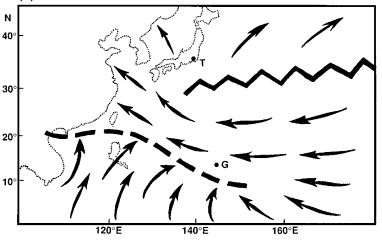
\includegraphics[width=20pc,angle=0]{H:/Documents/Admin/ESA/Figures/MT_Lander.png}
	\caption{Long-term average of the low-level circulation during the summer in the Tropics of the western North Pacific. Bold zig-zag lines indicate ridge axes, and the bold dashed line indicates the axis of the monsoon trough. Arrows indicate wind direction. The locations of Guam (G) and Tokyo (T) are indicated. Source: \cite{lander1996specific}}\label{fig:MT}
\end{figure}

% when does the MT vary?
The monsoon trough is a climatological feature of low pressure and convergence (figure \ref{fig:MT}), with increased vorticity and it exhibits substantial migrations and changes of shape \citep{lander1996specific}. When the monsoon trough is defined as the contiguous region where long-term (1988-2010) mean July-November 850 hPa relative vorticity is positive, 73\% of all July-November tropical cyclones form within the monsoon trough \citep{molinari2013percentage}. This percentage displays interannual variation correlated with Ni\~{n}o 3.4 index, with more TCs forming in the MT in an El Ni\~{n}o phase \citep{molinari2013percentage}. The shift in genesis with ENSO phase has been related to the eastward extension of the monsoon trough and westerlies (associated with the increased cyclonic low-level vorticity) and the reduction in vertical wind shear near the date line \citep{lander1994exploratory, lander1996specific, wang2002strong}.
%See Camargo funny summary paper.
%Atmosphere - monsoon trough and subtropical ridge are important.See Harr and Elsbery 1991, 1995, Lander 1994, 1996, Liu and Chan 2002.

The Madden-Julian Oscillation (MJO) is a tropical mode of variability that has an intraseasonal time scale (30-90 days). It is characterised by an eastward progression of large regions of both enhanced and suppressed tropical rainfall, observed mainly over the Indian and Pacific Ocean. Over the western North Pacific (WNP), tropical cyclone activity appears to be strong when MJO related convection centre is in the WNP \citep{kim2008systematic}, however, no significant relationship with intensity has been found \citep{liebmann1994relationship}. As well as affecting the preferable region for genesis, TC tracks respond to the large-scale steering flows related to the MJO. When convection is in the equatorial Indian Ocean, tracks migrate eastward and when over the tropical WNP, they migrate westward \citep{kim2008systematic}.


%, Kim et al 1996.
%correct? See paper: Schreck et al (2012) 80-95\% WPAC TCs form in direct association with active MJO and/or active regions of various equatorial waves. 

%Studies have shown that the westerly phase of the Quasi Biennial Oscillation (QBO) corresponds to a larger number of TCs (refs) due to a decrease in the upper-tropospheric vertical shear over the tropics during the boreal summer. But does not hold during El Ni\~{n}o (See Chan 1995).

The subtropical high and mid-tropospheric flow pattern are important to TC movement \citep{chan1982tropical}. The strength and extend of the subtropical high influence where a TC will recurve (\ref{fig:STH}). %(ref steering section). How changeable is the sth?

\begin{figure}[h]
	\centering
	\noindent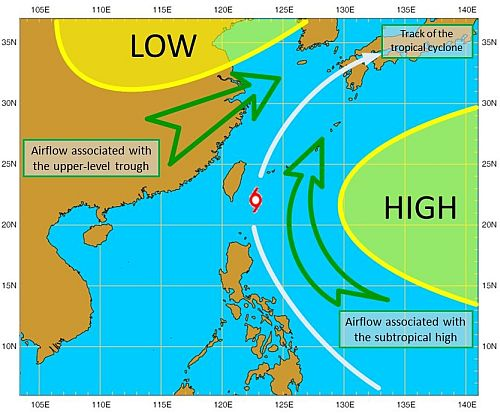
\includegraphics[width=16pc,angle=0]{H:/Documents/Admin/ESA/Figures/typhoon16_1e.jpg}
	\caption{Subtropical High influence on TC movement. Source: }\label{fig:STH}
\end{figure}
%source http://www.weather.gov.hk/education/edu01met/01met_tropical_cyclones/ele_typhoon16_e.html

The Pacific Decadal Oscillation (PDO) exhibits variations in North Pacific SST over a decadal (20-30 years) timescale. It is similar to ENSO, with positive and negative SST anomalies, although it is on a much longer time scale and the most pronounced variations are at high latitudes, rather than in the Tropics  (figure \ref{fig:PDO}). The PDO Index is defined as the leading principal component of North Pacific monthly sea surface temperature variability (poleward of 20N for the 1900-93 period) (http://research.jisao.washington.edu/pdo/). The PDO has a significant impact on the subtropical high and mid-level steering during the peak TC season. It creates a north-south dipole of geopotential height over the WNP, affecting the subtropical high extension and intensity as well as the zonal winds \citep{liu2008interdecadal}.
%Check out Ho et al 2004 for PDO.
%NB wind stress changes with changing SST


\begin{figure}[h]
	\centering
	\noindent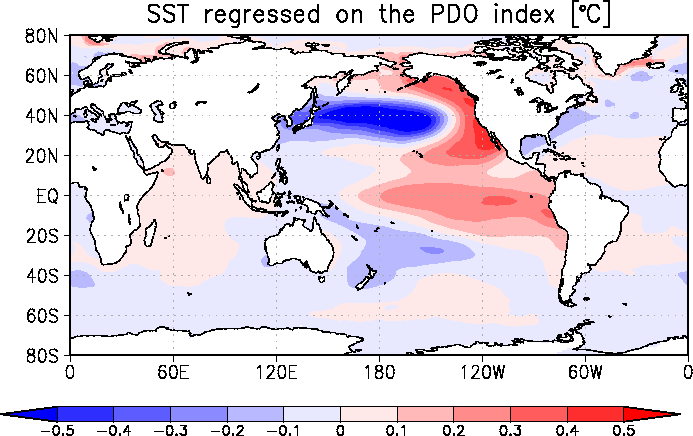
\includegraphics[width=20pc,angle=0]{H:/Documents/Admin/ESA/Figures/pdo_pattern.png}
	\caption{Pacific Decadal Oscillation (PDO) positive phase. Figure from ADD SOURCE }\label{fig:PDO}
\end{figure}
%Add source to above: http://ds.data.jma.go.jp/tcc/tcc/products/elnino/decadal/pdo_doc.html


%WPSH is highly predictable and this can be used for tropical storm predictions \citep{wang2013subtropical}.

%Modes of variability - see Zhan 2012 review.
%Steering - Harr and Elsberry - straight, recurving, recurving north.
%IOD
%The intensity of a given storm depends on its surrounding environment.
%wang2013subtropical - Indian Ocean refs.

%Know about tropical waves - see Lu seasonal paper.

%IO importance - on MT?

Natural climate variability strongly modulates the seasonal statistics of tropical cyclones. 

%Affect of cyclone beforehand - upwelling is negative, but wave train is positive? (See camargo1)
%No - do not need to cover everything about TCs. Be specific and relevant.
%Something about historic activity can be divided into clusters, for example Camargo, Chan.

\subsubsection{Long-term variability}

Warming of the climate system is unequivocal \citep{stocker2013ipccb}, and as the internal energy available to weather systems such as tropical cyclones changes, activity of these phenomena is also expected to change. Warming of the ocean accounts for 93\% of the increase in the Earth's energy between 1971-2010, with 64\% of this in the upper ocean (0-700 m) \citep{rhein2013chapter}.

Modelling studies have consistently projected that greenhouse warming is likely to cause increases in the global average intensity of tropical cyclones and related rainfall rates \citep[e.g.][]{hill2011impact, knutson2010tropical, elsner2008increasing, bender2010modeled}, but some suggest that this is still within the range of natural variability. Many studies have shown that with an increase in SST in the coming decades, tropical cyclones will have increasing wind speeds \citep{bender2010modeled, murakami2012future, webster2005changes, emanuel2005increasing, knutson2010tropical, elsner2008increasing}, with \cite{emanuel2005increasing} suggesting that for every increase in SST of 1$^{\circ}$C, peak wind speed would increase by 5\%. The assumption is that the dominant effect of increasing carbon dioxide on tropical cyclones is through an increase in tropical mean sea surface temperature \citep{zhao2013robust}. However, modelling studies show that both spatial patterns of sea surface temperature warming and higher atmospheric carbon dioxide affect tropical cyclones independent of global sea surface temperature warming. % (ref)
% refs for within range of variability.
%The observed warming of the tropics of around 0.5$^0$C over the past 4 to 5 decades \citep{wang2010climate}. Consensus that the amount of energy will be the same, but higher lats will be increasingly exposed? \cite{huang2015change} suggested a suppressive effect of subsurface oceans on TC intensity in a warming environment due to sharpening of the subsurface vertical temperature profile, and therefore stronger ocean coupling (cooling).

Alongside SST warming, the effect of global sea level rise has consequences for damage caused by tropical cyclones. Global sea level has risen 10 to 20cm over last 100 years \citep{solomon2007climate} and it is very likely that the rate of global mean sea level rise during the 21st century will exceed the rate observed during 1971-2010 \citep{church2013sea}, so tropical cyclone-induced storm surge will become increasingly damaging phenomena. The water-holding capacity of air is a function of temperature, approximately doubling with each 10$^{\circ}$C increase in the range -20 to +45$^{\circ}$C \citep{fowler1995potential}. Therefore, in a warmer climate, precipitation from tropical cyclones will likely be more intense.

%That this rclationship is translated into pre¢ipitation potential is •vidcnccd by satdlitc obscrvations rcported by St•phcns (1990), which show a comparablc non-lincar rclationship b•tw••n s•a-surface tcmpcraturc and prccipitablc watet in a vcrtical air column ovcr the o¢cans. \citep{fowler1995potential}

%A number of factors that a warmer climate will affect on the activity and impact of tropical cyclones.

%Does it matter than here talking about modelling studies, before have talked about TCs in GCMs?

\section{Observations of tropical storms}
The historic record of tropical storm activity is longest for the North Atlantic, where records start in 1851 \citep{landsea2004atlantic}. Over the following decades, there has been a significant change in the methodology used to record such storms. In the early period, the main method for identifying tropical cyclones was by records of landfalling storms or by records of ships at sea \citep{vecchi2008estimates}. Further back in time, there were fewer ships and shipping lanes as well as fewer people living in the tropical and subtropical coastal regions \citep{landsea2007counting}, therefore it was possible that many storms were unrecorded. Aircraft reconnaissance in the West Pacific began near the end of the second World War and ended in 1987 \citep{knapp2013pressure}, and since then tropical storms have been monitored primarily by satellite \citep{lander1994exploratory}. The need for increased aircraft reconnaissance is acknowledged throughout the research and operational communities, with a recommendation from the World Meteorological Organisation (WMO) to 'realize the goal of regular and coordinated aircraft reconnaissance in the western North Pacific and other TC basins' \citep{wmoitwc8}. As part of government-led research, Japanese researchers are planning to have aircraft reconnaissance in the WNP from 2017 to at least 2020 \citep{nhkhurricanehunter}.

%, as many tropical cyclones(remove?)  were likely undetected over the tropical ocean in the pre-satellite era \citep{camargo2007cluster}

It is well established that although records begin many decades ago for some basins, they are only really trusted since the satellite era, ie. around the 1970s \citep{landsea2007counting} when global observations were possible. The observed time series of WNP tropical cyclone activity appears to be affected by artefacts of the changing observing system  \citep{lander1994exploratory, knapp2013pressure}, including the increasing use of satellite data and refining these methods, e.g. the Dvorak technique.
% and procedural changes . \citep{schreck2014impact} \citep{knapp2010international}

There are a number of agencies that produce Best Track records of tropical storm activity. The  International Best Track Archive Climate Stewardship (IBTrACS)\citep{knapp2010international} database consists of data from the World Meteorological Organization (WMO) Regional Specialized Meteorological Centres (RSMC) and Tropical Cyclone Warning Centres (TCWC) \citep{knapp2010international}. In the West Pacific region, data from the following agencies is available:

\begin{itemize}
	\item Fiji Meteorological Service (as RSMC Nadi)
	\item Japan Meteorological Agency (JMA) (as RSMC Tokyo)
	\item China Meteorological Administration’s Shanghai Typhoon Institute (CMA/STI)
	\item Hong Kong Observatory (HKO)
	\item U.S. Department of Defense Joint Typhoon Warning Center (JTWC)
\end{itemize}

For the WPAC region, JTWC storm data is most widely used \citep{knapp2010international}. All of the other agencies in this list provide data for a specific region in the West Pacific, rather than covering the entire basin. In some cases the same storms are tracked by multiple agencies, large differences in intensity can be found. There are also differences in lifetime as agencies employ different procedures for deciding when the first and last track point are determined.

%Modelling studies are vital, to learn more about TCs in the current climate and also to explore potential changes in the future.
% (tracks generallyu ok?), Also differences in lifetime - keep recording when goes ET or moves out of area of interest? Landfall in China goes further in CMA dataset (Matthias, pers comm). Different tracks, intensities, lifetime. eg. differences if calculating ACE. (see zhan2016cfs) Historical pressure record is more consistent between agencies than wind reports \citep{knapp2013pressure}.


\section{Representation of tropical storms in models}

\subsection{Global climate models}

Current CMIP5 (Coupled Model Intercomparison Project 5) models assessed in the IPCC Fifth Assessment Report (AR5) have a finest horizontal resolution in the atmosphere of around 70km, but the average is about 200km \citep{climodaus}, an increase from the previous four versions of the report.
It is well established that the current generation of global climate models (GCMs) are of insufficient resolution to simulate tropical cyclones in detail due to their low resolution in comparison to the size of the storm core \citep{lin2012physically} and the complex nature of tropical cyclone structure, although enhanced computing capabilities and parametrisations have resulted in better representation of tropical cyclones \citep{zhao2009simulations, bengtsson2007may, walsh2007objectively}.

Modern GCMs are capable of producing structures that can be recognized as similar to tropical cyclones at resolutions as coarse as 100 km (Knutson et al. 2010), but without the details of the core \citep{mcdonald2005tropical}. There is a need for very high resolution in order to simulate realistic storm intensities, \citep{bender2010modeled, emanuel2008hurricanes} for example it has been suggested that 2 km or less is needed to represent important physical processes in the tropical cyclone eyewall \citep{gentry2010sensitivity}, with \cite{chen2007cblast} suggesting that a resolution of 1 km is required to resolve hurricane eye wall convection and wind maxima.
%  (not realistic for GCM? Talking about RCM?)


Resolution is important for simulating storm intensity, but less critical for simulating the annual number of tropical cyclones and their geographical distribution. \cite{zhao2009simulations} found that a model with a resolution in 20-100km range was able to simulate climatology and interannual variability of tropical storm frequency without realistic distribution of storm intensity. Similar results were found by \cite{strachan2013investigating}, with realistic interannual variability of storm occurrence requiring resolutions of 100 km or higher, but skill was basin dependent. Different models produce substantially different annual global tropical cyclone frequencies and geographical distributions due to model resolution and physical parametrisations \citep{zhao2013robust}. It has been found that there are larger differences in tropical cyclone distribution between models than in the same model at different resolutions, suggesting a greater influence of model specifics than resolution \citep{shaevitz2014characteristics}.
%60km, 25 km, 12 km (NWP size).


%\subsection{Regional models}

%Regional models can be run at higher resolution than global models due to the reduced area over which calculations are being made. Typical resolution is ... and can be embedded in GCMs or GCMs downscaled.


%\newpage


\section{Seasonal prediction of tropical storm activity} % changed this from chapter to section

\subsection{Tropical storm forecasting techniques} % prediction?

%Remember focussing on climate, not NWP

The atmosphere is a chaotic system and so determinisitic predictability of weather phenomena, for example, tropical cyclones, is limited, and on a seasonal time scale, impossible. However, rather than forecasting exact cyclone tracks and dates of occurrence, predictions are made for basin-wide activity over a seasonal period.
Seasonal predictability of the climate system stems from the slowly evolving lower boundary, e.g. ocean forcing. The balance between the oceanic forcing and effects of random chaotic weather therefore determine the level of seasonal skill over a region \citep{rowell1998assessing}, and On a seasonal scale, atmospheric potential predictability is highest over the tropical oceans, where SST has an important effect, and this can be predicted using dynamical or statistical models \citep{rowell1998assessing}.
Seasonal tropical storm predictions are developed using dynamical, statistical, or statistical-dynamical models, with forecasts typically made 3 months ahead, e.g. March for the start of the season in June, with updated in May or June. 

%The time scales of changes in the ocean are much slower than in the atmosphere and can provide a source of predictability (e.g. ENSO). 
%The climate exhibits non-linear behaviour on a range of time scales, which may limit the seasonal climate predictability \citep{zhan2012seasonal}.
%, Palmer 2006.

%\begin{figure}[h]
%	\centering
%	\noindent\includegraphics[width=30pc,angle=0]{H:/Documents/Admin/ESA/seasonalforecasts.png}
%	\caption{Seasonal forecasts from different agencies. Most recent hurricane forecasts from each of the forecasting centers. Limits for the activity levels correspond to the ones defined by NOAA. Source: \citep{seasonalhurr}}\label{fig:seasonalforecasts}
%\end{figure}


%\begin{figure}[h]
%	\centering
%	\noindent\includegraphics[width=16pc,angle=0]{H:/Documents/Admin/ESA/na_ts_forecast_sm11.png}
%	\caption{Met Office seasonal forecast for North Atlantic. Also Hurricanes and ACE plots. None for the West Pacific yet as lacking skill. http://www.metoffice.gov.uk/weather/tropicalcyclone/seasonal/northatlantic2016}\label{fig:seasonalforecasts2}
%\end{figure}


%Predictable to some extent on seasonal time scale, but with large uncertainties. 
%predictability of large-scale environment


\subsection{Dynamical modelling}

In climate models accurate representation of the ocean is vital for climate simulation, especially over long periods, as the ocean represents a dynamic thermal reservoir that exchanges energy with the atmosphere. Fully-coupled atmosphere-ocean models, where heat and transport are fully represented and interactive, provide the best opportunity to capture relationships at a variety of scales.  These global models are vital as they can capture teleconnections, which are important for seasonal prediction. However, these are run at too coarse a resolution to capture the intensity. Model intensities are often not used directly, and instead are compared to the model climatology, which is then adjusted to cover the full spectrum of intensities. In order to extract the storms, a tracking algorithm needs to be applied to the model output. There are various different methods, for example tracking vorticity or minimum pressure, and then further thresholds are applied to select only tropical storms (e.g. warm core). %Tracking algorithms are not the same - not the same output storms, but with increasing resolution are better. Horn et al - thresholds. Basin-wide storm activity, released MAM? update June?


The skill of seasonal forecast models is often found to be higher using an ensemble than any single deterministic run \citep[e.g.][]{vitart2006seasonal}, and ECMWF use this ensemble approach. Dynamic models are important to explore the future climate, as long as they have sufficient skill at simulating the present climate and future forcings.

Seasonal forecasts for WNP tropical cyclone activity from dynamical models are produced by the European Centre of Medium-range Weather Forecasting (ECMWF). They have produced operational seasonal tropical cyclone forecasts for all basins since 2001 with their global coupled model. Predictions include tropical storm frequency, typhoon frequency, track density and accumulated cyclone energy (ACE) \citep{zhan2012seasonal}.

% Ensembles better than deterministic - see molinari cfs paper

%IRI uses\ a two step approach, whereby first SSTs are predicted using statistical or dynamical models, then atmospheric models are forced with these \citep{camargo12007seasonal}. IRI issues ACE forecast. IRI are probabilistic, normal , above normal, below normal \citep{camargo12007seasonal}. In both cases, TCs then tracked.
%ECMWF resolution
%IRI hybrid?????? , and the International Research Institute for Climate and Society (IRI). 
%Importance of ocean and ENSO prediction (refer to enso section). ENSO on SST field, but also on atmospheric pattern. Seasonal prediction of tc landfall represents a major challenge for dynamical models \citep{camargo12007seasonal}.\\
%\citep{rowell1998assessing} GCM skill in potential predictability
%\citep{vitart2006seasonal}
%\citep{mcdonald2005tropical}
%\citep{shaevitz2014characteristics}

%Limits of dynamical models for seasonal forecasting:
% \begin{itemize}
%	\item Resolution insufficient to capture storm structure and intensity (BUT there can be regional or hi res global dynamical models too?)
%	\item Global teleconnections need to be represented (and are they not?)
%	\item Model biases are present, which need to be corrected for
%	\item Limitations of the tracking methodologies (only apply to dynamical models?)

%\end{itemize}


%What are plans for operational - future - higher res, ensembles, physics problems to solve
%Landfall forecasts
%Modes of variability are important - teleconnections, also processes in the cryosphere, land, stratosphere, ocean, need fully coupled global  model.
%GloSea5, ECMWF and local models.
%bogussing? 

%basin wide and lead time 

\subsection{Statistical models}  
It has long been established that large-scale variability affects tropical cyclone activity globally. If a robust relationship between large-scale predictors and this activity can be found, it is possible to make predictions about future activity using statistical analysis.

The first region over which a statistical forecast for tropical cyclone activity was produced was the Australian region, in the late 1970s and 1980s \citep{nicholls1979possible, nicholls1985predictability}, with forecasts for the North Atlantic starting in 1984 \citep{gray1984atlantic}.

The first operational tropical cyclone forecasts for the West Pacific were issued by the National Climate Center (NCC) or CMA (China Meteorological Agency) in 1994 but these were only available in China \citep{zhan2012seasonal}. NCC currently issue seasonal forecasts of WNP tropical cyclone activity in March, with updates in June. The predictors are ENSO index, 500 hPa geopotential height over the Pacific and Australian region, convective activity over the WNP, vertical wind shear of zonal wind over the WNP and tropical eastern Pacific prior to the season \citep{zhan2012seasonal}.% EPAC Matters?

In 1997, The City University of Hong Kong, China (CUHK) started to issue seasonal forecasts to the public.  This scheme used SST anomalies as a proxy for ENSO signal, the large-scale circulation over Asia and the western Pacific, and trend or climatology and persistence \citep{chan1998seasonal}. New predictors related to ENSO including changes to the Southern Oscillation, Australian monsoon and subtropical high in the South Pacific have since been identified \citep{cl2001improvements}.
%persistence?
%Also did landfall in South China and Korea and Japan in 2009 and 2010 - still going?
%What is the CSL scheme? Does it stand for something? Not mentioned in the paper in 1998 - this is the one that details the model first used in 1997.
%(CHUK forecast 1997 or check this - is it 2000) The CSL scheme proposed by Chan et al 1998 
%.Relationship with the southern hemisphere related to the La Ni\~{n}a cold event.
Previous work by \cite{lu2013seasonal} examined the seasonal predictability of tropical cyclones affecting Taiwan using an empirical model. They found some skill in predicting accumulated cyclone energy (ACE) in the peak season (JJAS) using the SST in three regions and the sea level pressure (SLP) over an area in East Asia as predictors. 


%based on scientific understanding of the oceanic and atmospheric influence on tropical cyclones.
%Talk about verifying model using same dataset and similar region over Taiwan. Extending region to include more landfalling storms.

%Alongside CUHK and NCC, Tropical Storm Risk (TSR) also issue a statistical forecast for the WNP.
%statistical forecasts from CityU, National Climate Center China (NCC), Tropical Storm Risk (TSR) for the WNP. 

%Using a multivariate linear regression procedure, some skill is found using 3 regions of sea surface temperature and one region of sea level pressure predictors in forecasting the ACE over Taiwan. 
%Usually issued in March or April, with update in June or July.
%Seasonal statistical model - predictability from the spring to summer evolution of the monsoon subtropical high-ENSO system in association with the evolution of the Indo-Pacific SST anomalies \citep{lu2013seasonal}.

%Statistical modelling section - can also use statistical models of the large-scale environment to predict storm intensity distribution \citep{lee2015probabilistic}.
%Estimating or predicting landfall is important. Can create genesis models, track models etc. all from large-scale environment.

Limitations of such statistical forecasts include the dependence on historic observed data. this data is relatively limited (50 years) and has associated biases and errors. They assume stationarity of relationships and are unable to be used for climate change projections.
%Need to have cross correlations. Climate projections are difficult as rely on the signal at present (and in historic record).

%Limitations of statistical models for seasonal forecasting:
%\begin{itemize}
%	\item Dependent on historic observed data (limited and short record)
%	\item Climate projections difficult as future projections rely on present signal
%	\item Often assumes stationarity in relationships

%\end{itemize}

Alongside statistical and dynamical approaches, hybrid statistical-dynamical approaches have increased in popularity in recent years.

\subsection{Hybrid dynamical-statistical models}  
These models are a combination of the dynamical and statistical modelling approaches. A statistical model is developed based on either observations or output from a climate model seasonal prediction, and then this is applied to the seasonal prediction using predictors from a dynamical model. Skill of this model depends on robustness of the statistical relationship as well as the skill of the model to predict the predictor. \cite{zhan2016cfsv2} showed that a hybrid dynamical-statistical model showed better skill at longer lead times that the pure statistical model at predicting seasonal accumulated cyclone energy (ACE).
%BUt this PHd will focus on statistical?
% stationarity

%Quick summary sentence about timing of the forecast.
%ENSO predictability follows a cycle, where state for 4-6 months can be relatively accurately predicted between July and November \citep{camargo12007seasonal}. Once an episode has begun, predicting its continuation for the next 9-12 months is much easier than predicting its initial appearance \citep{camargo12007seasonal}.

%Relate this to TC season and timing of forecasts.

%\subsubsection{Seasonal forecast verification}  

%Previous studies have created statistical models of ACE or other tropical storm diagnostics such as frequency etc. (eg. Chan, Lu), and here we add to this by including the sub-surface ocean state in terms of ocean heat content and tropical cyclone heat potential.ADD LANDFALL
%provides more information over the depth of the ocean, important for intensity of the storms (ref intro).

Most seasonal projections are basin-wide. Here, we explore seasonal forecasts for a specific region of landfall and utilise current reanalysis datasets, including data on the deeper ocean. We also extend the lead time of predictability into the previous 15 months before the season.%....... Lu at al did the Taiwan region 6 months in advance. Others have focussed on basin-wide forecasts. EXTEND

%%%%%%%%%%%%%%%%%%%%%%%%%%%%%%%%%%%%%%%%%%%%%%%%%%%%%%%%%%%%%%%%%%%%%%%%%%%%%%


%How does my work compare to what has already been done.



